\documentclass[xcolor=dvipsnames,11pt]{beamer} 

\mode<presentation>
{
\usetheme{Malmoe}
\useinnertheme{rounded}
\usecolortheme{beaver} 
\usecolortheme[named=Mahogany]{structure} 

\setbeamertemplate{navigation symbols}{}%remove navigation symbols
}

\usepackage[utf8]{inputenc}
\usepackage[english]{babel}

\usepackage{amsmath}
\usepackage{amsfonts}
\usepackage{amssymb}

\usepackage{graphicx}
\usepackage{xspace}

% \usepackage[dvipsnames]{color} loaded by beamer, see above

\usepackage{listings}

%%%%%%%%%%%%%%%%%%%%%%%%%%%%%%%%%%%%%%%%%5
\newcommand{\comment}[2]{{\tiny \color{Orange}{$\spadesuit${\bf #1: }{\sf #2}$\spadesuit$}}}
%\renewcommand{\comment}[2]{}

\newcommand{\jbcomment}[1]{\comment{JB}{#1}}
\newcommand{\pbcomment}[1]{\comment{PB}{#1}}
\newcommand{\mecomment}[1]{\comment{ME}{#1}}

%%%%%%%%%%%%%%%%%%%%%%%%%%%%%%%%%%%%%%%%%5
\lstloadlanguages{Haskell,C}
% auto-colorisation with listings, handy for known languages...
\lstdefinestyle{hsstyle}{
  language=Haskell,
  basicstyle=\scriptsize\rmfamily,
  commentstyle=\it\color{Green},
  stringstyle=\mdseries\rmfamily\color{Gray},
  showspaces=false,
  showstringspaces=false,
  keywordstyle=\bfseries\rmfamily\color{Violet},
  morecomment=[l]{--},
  morecomment=[s]{\{-}{-\}},
  literate={+}{{$+$}}1 {/}{{$/$}}1 {*}{{$*$}}1 {=}{{$=$}}1 {>}{{$>$}}1 {<}{{$<$}}1 
           {\\}{{$\lambda$}}1
           {\\\\}{{\char`\\\char`\\}}1 {|}{{$\mid$}}1
           {->}{{$\rightarrow$}}2 
           {\\n}{{\textbackslash n}}2 
           {>=}{{$\geq$}}2 {<-}{{$\leftarrow$}}2
           {<=}{{$\leq$}}2 {=>}{{$\Rightarrow$}}2
           {\ .}{{$\circ$}}2 {\ .\ }{{\ $\circ$\ }}2
           {>>}{{>>}}2 {>>=}{{>>=}}2
  ,    
%  columns=flexible,
  emphstyle={\bf},
  mathescape,
% specific to this presentation: contract language keywords and types
  emphstyle={[5]\color{Brown}\textbf},
  emph= {[5]
         zero, transfOne, scale, transl, both, iff, checkWithin,
         both, acc, obs, chosenBy, maxx, minn,
         RealE, BoolE, Expr, Party, Contract, MContract, Env, MEnv,
         Currency, EUR, USD, SEK
	    },
}
\lstnewenvironment{hscode}
   {\lstset{basicstyle=\scriptsize,style=hsstyle,frame=tlrb}}
   {}
\lstnewenvironment{hscodesmall}
   {\lstset{basicstyle=\tiny,style=hsstyle,frame=tb}}
   {}
\lstset{style=hsstyle,keepspaces=true,breaklines=false}\newcommand{\cd}[1]{\lstinline$#1$}

%%%%%%%%%%%%%%%%%%%%%%%%%%%%%%%%%%%%%%%%%%
\renewcommand{\emph}[1]{\textcolor{structure!90}{#1}}

%%%%%%%%%%%%%%%%%%%%%%%%%%%%%%%%%%%%%%%%%%%%%%%%%%%%%%%%

% change here to change all
\newcommand{\ttt}[1]{\mbox{\cd{#1}~}}

% smart constructors
\newcommand{\zero}{\ttt{zero}}
\newcommand{\transfOne}{\ttt{transfOne}}
\newcommand{\scale}{\ttt{scale}}
\newcommand{\transl}{\ttt{transl}}
\newcommand{\both}{\ttt{both}}
\newcommand{\ifff}{\ttt{iff}}
\newcommand{\checkWithin}{\ttt{checkWithin}}

\title{Small Symbolic Multi-Party Contracts}
\author[Bahr,Berthold,Elsman,Henglein]{Patrick Bahr, Jost Berthold, Martin Elsman, Fritz Henglein}

\begin{document}

\frame[plain]{\titlepage}

%\section{Motivation}

\begin{frame}
    \frametitle{Models, contracts, pricing, risk analysis}

\begin{columns}
\column{0.5\textwidth}
\emph{\textsc{Hiperfit} key ideas}

\begin{itemize}
\item DSL technology
\item Modular architecture
\item Separate parts: models, contracts, engines
\end{itemize}
\column{0.4\textwidth}
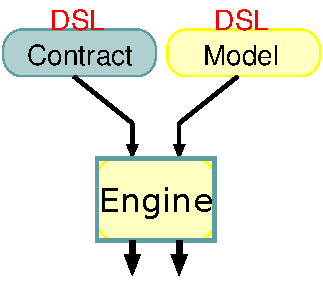
\includegraphics[width=1.1\textwidth]{DSLvision}
\end{columns}

\begin{itemize}
\item Experiment in \emph{contract modelling}:

\emph{enabler} for \emph{risk analysis} and other \emph{symbolic manipulation}
\item Overall goal: \emph{create our own \textsc{Hiperfit} infrastructure/suite}
\end{itemize}

\end{frame}

\begin{frame}[fragile,t]
    \frametitle{Contract Language Goals}

\begin{itemize}
\item \emph{\textbf{Compositionality}}. 

Contracts are time-relative $\Rightarrow$ straightforward compositionality

\item \emph{\textbf{Multi-party}}.

Specify obligations and opportunities \emph{for multiple parties},
(which opens up the possibility for specifying portfolios)

\item \emph{\textbf{Contract management}}.

\emph{Contracts} can be managed and \emph{symbolically evolved};\\
a contract gradually reduces to the empty contract.

\item \emph{\textbf{Contract utilities (symbolic)}}.

Contracts can be analysed in a variety of ways

\item \emph{\textbf{Contract pricing (numerical, staged)}}.

Code for payoff can be generated from contracts

(\emph{input} to a stochastic \emph{pricing engine})

\end{itemize}

\end{frame} 

%\section{Appearance and (intuitive) semantics}

\begin{frame}[fragile,t]
    \frametitle{Simple examples}

\emph{Vanilla option on Carlsberg stock}
\begin{hscodesmall}
callOption = scale 1000 -- nominal
              (transl maturity
                  (scale carlsb (transfOne EUR "DB" "me"))))
  where maturity = oneYear -- == 365, using ACT/365
        strike  = 50.0
        carlsb  = maxx 0.0 (obs ("Carlsberg",0) - strike)
\end{hscodesmall}

\emph{FX barrier touch option on EUR/USD rate}
\begin{hscodesmall}
barriertouch
  = checkWithin (1.0 !<! obs ("FX EUR/USD",0)) oneYear
                (scale 1000.0 (transfOne EUR "Nordea" "you"))
                zero
\end{hscodesmall}

\begin{itemize}
\item Note: \emph{observables} - anything, \emph{transfers} - defined assets (type)
\item Multiparty: seller and buyer perspective only suggested by "you" and "me" strings
\end{itemize}

\end{frame}

\begin{frame}[fragile,t]
    \frametitle{A complex OTC barrier touch option}

\begin{hscodesmall}
barrierRevConvert :: MContract -- managed contract
barrierRevConvert
   = (at "2012-01-27", -- contract start date
      iff breached (transl 367 
                    (iff (oneBelow 1)
                         (collectEUR minRatio) (collectEUR 1000))
                   zero) where 
  idxs   = [ "DJ_Eurostoxx_50", "Nikkei_225", "SP_500" ]
  spots  = [ 3758.05, 11840, 1200 ]
  oneBelow d = foldl1 (!|!) (zipWith (cmpFrac d) idxs spots)
  cmpFrac d idx spot = obs(idx, 0) !<! d * spot
  minRatio = foldl1 minn 
              (zipWith (\id sp -> obs(id,0) / sp) idxs spots)
  breached = acc (\x -> x !|! oneBelow 0.7) 366 (oneBelow 0.7)
  collectEUR amount = scale amount (transfOne EUR "them" "us")
\end{hscodesmall}

\begin{itemize}
\item barrier of $0.7 \cdot \ttt{spot}$ on 3 indexes, monitored over 367 days;
\item payment if barrier breached, scaled if at least one end index lower than start


\end{itemize}
\end{frame}

%\begin{frame}[fragile,t]
%    \frametitle{Observable Environments}
%
%\begin{hscode}
%-- environment: maps (observable,day) to possible value
%type Env = (String, Int) -> Maybe Double
%-- managed environment
%data MEnv = Env Date Env -- environment and start date
%
%emptyFrom :: Date -> MEnv -- construct empty mgd. env.
%
%-- add values to the environment
%addFixing :: (String, Date, Double) -> MEnv -> MEnv
%addFixings :: (String, Date) -> [Double] -> MEnv -> MEnv
%
%-- construct an environment from given start date and values 
%fixings :: String -> Date -> [Double] -> MEnv
%fixings s d vs = addFixings (s,d) vs (emptyFrom d)
%
%-- translate an environment in time
%promoteEnv :: MEnv -> Int -> MEnv
%\end{hscode}
%
%\begin{itemize}
%\item Environments store information about observables
%
%\item Contracts are \emph{symbolic} (they do not model observables)
%
%\item Environments can/should be constructed from models
%\end{itemize}
%
%\end{frame}

\newcommand{\crule}[3]{\frac{#2}{#3}\ \mbox{\scriptsize \it #1}}
\newcommand{\sem}[1]{[\![#1]\!]}
\newcommand{\csem}[3]{\mathcal{C}\sem{#1}#2 & = #3}

\begin{frame}[fragile,t]
    \frametitle{Formal Semantics: Sequence of Cash Flow Sets}

\emph{Environment}: information about observables and choices

 (Contracts are \emph{symbolic}, they do not model observables)
\begin{hscode}
-- internal environment with relative time
type Env = (String, Int) -> Maybe Double -- also choice

data MEnv = E Date Env -- managed env, with start date
\end{hscode}

\emph{Semantics of an expression}: (partially) defined 
wrt. an environment ($\ttt{Env}$), containing fixings for
observables and choices:

%\vspace*{-2ex}

{\footnotesize
$$
  \mathcal{E}_a : \ttt{Expr a} \times \ttt{Env} \not\longrightarrow \ttt{a}
$$}
\vspace*{-2ex}

\emph{Semantics of a contract}: (partially) defined wrt.
an environment, as a series of cash flow sets:

$$ \mathcal{C} : \ttt{Contract} \times \ttt{Env} 
          \not\longrightarrow \mathbb{P}(\ttt{Flow})^\mathbb{N}$$
\vspace*{-2ex}

\emph{Cash flow}: \cd{Flow \{amount::Double, c::Currency, from::Party, to::Party\}}.

\end{frame}

\begin{frame}[t] \frametitle{Some contract equivalences}

\emph{\textbf{Expression promotion:}}

Expressions involving observables can be \emph{promoted} from a time later to a time earlier:
%
\hfill {\footnotesize $(e \in \ttt{Expr a},\ d \in \mathbb{Z})$}

{\footnotesize 
$$ e / d = \left \{
\begin{array}{ll}
obs(s,\emph{d+i}) :& e = \emph{obs(s,i)}\\
e_1/d \oplus e_2/d :& e = e_1 \oplus e_2\\
\ldots
\end{array}
\right .$$
}

An expression is \emph{certain} if it does not depend on observables.
\medskip

\hrule
\medskip

\emph{\textbf{\ldots enables equivalences with \cd{transl}}}

{\footnotesize
\begin{align*}
    \transl d~ (\scale s c)       &=  \scale (s/d) ~(\transl d c)\\
    \transl d~ (\scale s c)       &=  \scale s~ (\transl d c)\  \mbox{if } s \mbox{ is certain}\\
%
  \transl d~ (\checkWithin b ~ e  ~c_1 ~c_2)  &=  \\
                             \checkWithin &(b/d)~ e~ (\transl d ~c_1) ~(\transl d ~c_2)\\[1ex]
  \transl d~ (\ifff b~ c_1 ~c_2)  &= \ifff (b/d)~ (\transl d ~c_1)~ (\transl d ~c_2)\\
\end{align*}
}

\end{frame}

%\section{Analysis and manipulation}

\begin{frame}[fragile,t]
    \frametitle{Contract transformation using environment information}

\emph{Evaluating a contract (scaling, branching) as far as possible}
\begin{hscode}
-- reduce a contract, using available values in environment
simplify :: MEnv -> MContract -> MContract
\end{hscode}

\emph{Example:} Barrier option with known fixings simplifies to cashflow

\hrulefill

\emph{Eliminating branches in a contract (not applying scaling)}
\begin{hscode}
-- eliminate all branches which are known to not be taken
elimBranches:: MEnv -> MContract -> MContract
\end{hscode}

useful for scenario generation
\end{frame}

\begin{frame}[fragile,t]
\frametitle{Example Portfolio of Touch Options}

\begin{hscodesmall}
touchOptions -- :: MContract, pair of date and contract
  = (today, allCs
     [ fxTouch   "C" "us" USD   40000 (USD,SEK) 6.90 Up   halfY
     , fxTouch   "D" "us" USD   60000 (USD,SEK) 6.15 Down oneY
     , fxNoTouch "A" "us" USD  140000 (USD,SEK) 6.70 Up   halfY
     , fxNoTouch "B" "us" USD  160000 (USD,SEK) 6.25 Down oneY ])
env = fixings "FX USD/SEK" today
      [6.6,6.7,6.8,6.9,6.8,6.7,6.6,6.5,6.4,6.3,6.2,6.1]

allTouch' = simplify env touchOptions
\end{hscodesmall}

{\scriptsize
Two touch options will be triggered (barriers up 6.9, down 6.15).

Two no-touch options will be canceled (barriers up 6.7, down 6.25).
}
\vfill
\emph{Result:} 
{\small
\begin{verbatim}
 *Main> (putStrLn . ppCashflows . cashflows) allTouch'
 2014-01-03 Certain [C->us] USD 400000.0
 2014-01-11 Certain [D->us] USD 600000.0
\end{verbatim}
}
\end{frame}

\begin{frame}[fragile]
\frametitle{Contract analysis: finding branch boundaries}

\begin{hscode}
data Trigger = Trigger { underlying :: String
                       , start :: Int, end :: Int
                       , values :: [ Double ] }
-- | find all branch boundaries for a contract
branchBounds :: MContract -> [ Trigger ]
\end{hscode}

\begin{itemize}
  \item Finds all observables which occur inside conditionals

      \emph{Goal:} generate tree of scenarios with fixings.
      
   \item A \cd{Trigger} is an \emph{observable} and \emph{its boundary values}
       for a certain \emph{time range} within a contract horizon.

\end{itemize}

\emph{Example:} our touch options from before
{\small
\begin{verbatim}
  *Main> (putStrLn . ppTriggers . branchBounds) touchOptions
  FX USD/SEK from day 0 to 182: 6.1500, 6.2500, 6.7000, 6.9000
  FX USD/SEK from day 183 to 365: 6.1500, 6.2500
\end{verbatim}
}

\end{frame}


%\section{Next steps and vision}

\begin{frame}
    \frametitle{Next steps and vision}

\emph{Payoff code generation} for arbitrary OTC contracts

\begin{columns}
\column{0.6\textwidth}
\begin{itemize}
\item connect contracts framework to generic pricing [FHPC'12]

\item bridging from symbolic manipulation to numerical and stochastic valuation
\end{itemize}
\column{0.35\textwidth}

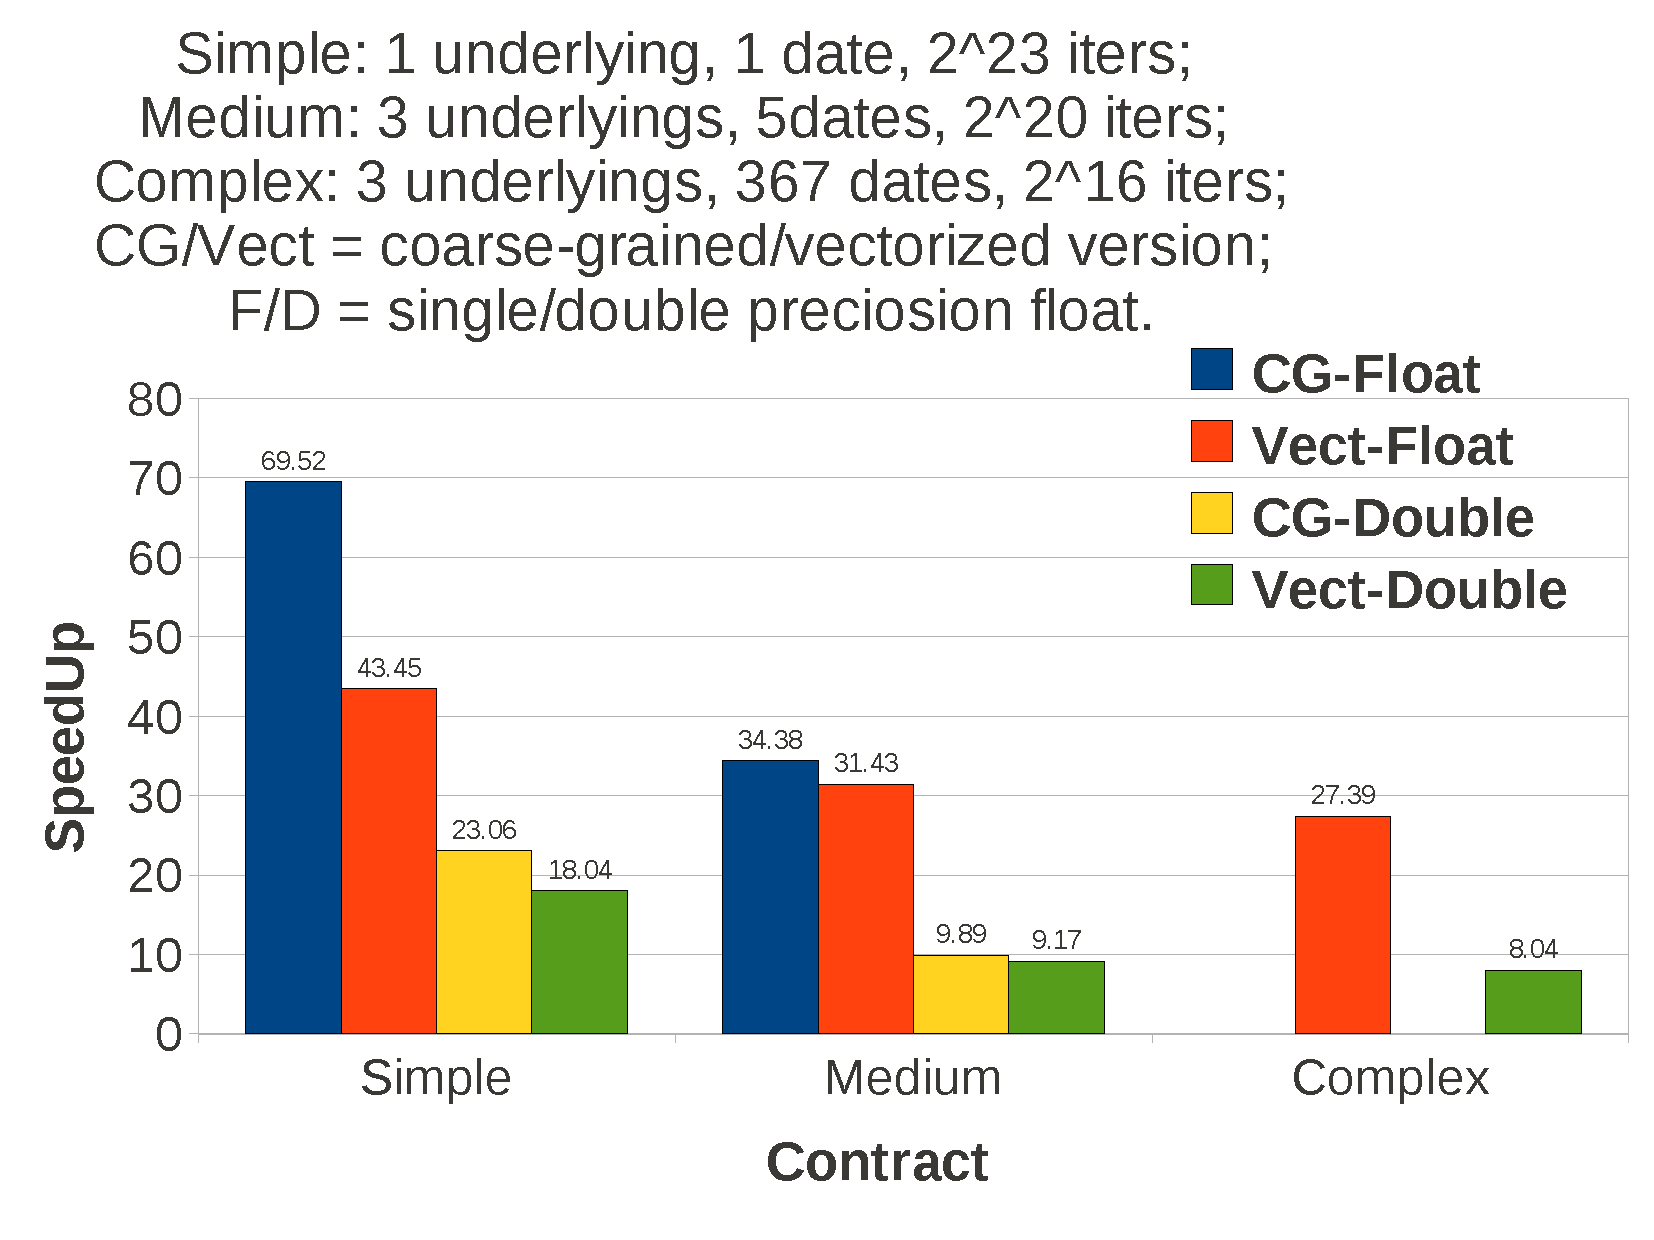
\includegraphics[width=1.2\textwidth]{SpeedUpNewFig}
\end{columns}
\medskip
\hrulefill

\emph{Risk analysis} by symbolic scenario generation
\begin{itemize}
\item based on decision triggers in conditional contracts
\item providing input for hedging efforts
\end{itemize}

\end{frame}


\frame{\huge \centering \emph{\bf Appendix}\\}

\begin{frame}[fragile,t]
    \frametitle{Expressions and Intuitive Semantics}

\begin{hscode}
data Expr a where
    I :: Int    -> Expr Int    -- Int
    R :: Double -> Expr Double -- Double
    B :: Bool   -> Expr Bool   -- Bool
    V :: Var    -> Expr a      -- Variable
-- | arithmetic operations: + - * / max min
$\oplus$ :: Num a => Expr a -> Expr a -> Expr a
-- | logical operations: < = ! |
!<! :: Ord a => Expr a -> Expr a -> Expr Bool
!=! :: Eq a  => Expr a -> Expr a -> Expr Bool
not :: Expr Bool -> Expr Bool
!|! :: Expr Bool -> Expr Bool -> Expr Bool

type RealE = Expr Double; type BoolE = Expr Bool
\end{hscode}

\begin{description}
\item[I d] is the integer constant $d$.
\item[R r] is the real (i.e., double) constant $r$.
\item[$e_1 \oplus e_2$] is transformed automatically (ad-hoc polymorphism)
\item[$e_1 !\!\!<! e_2$] compares embedded values (includes evaluation)
\end{description}

\end{frame}

\begin{frame}[fragile,t]
    \frametitle{Expressions and Intuitive Semantics (2)}

\begin{hscode}
data Expr a where
    -- continued...
    -- Observables and choice
    obs :: (String, Int) -> Expr Double    -- observable
    chosenBy :: (String, Int) -> Expr Bool -- choice

    -- Accumulator. acc(f,i,a) := f/i(...(f/2(f/1(a))))
    acc :: (Expr a -> Expr a) -> Int -> Expr a -> Expr a

    -- Pairs
    pair :: Expr a -> Expr b -> Expr (a,b)
    fst :: Expr (a,b) -> Expr a
    snd :: Expr (a,b) -> Expr b
\end{hscode}

\begin{description}
\item[obs(s,d)] represents the value of the underlying ``s'' in $d$ days.
\item[chosenBy(s,d)] represents a choice made by party ``s'' in $d$ days.
\item[acc f i a] accumulates a value for $i$ days using $f$, starting with $a$
\end{description}

\end{frame}

\begin{frame}[fragile,t]
    \frametitle{Contract Constructors and Intuitive Semantics}

\begin{hscode}
  data Currency = EUR | USD | SEK... -- names (assets)
  type Party = String       -- parties
  data Contract -- internal -- contracts
  zero        :: Contract            
  transfOne   :: Currency -> Party -> Party -> Contract
  scale       :: RealE-> Contract-> Contract
  transl      :: Int-> Contract-> Contract
  both        :: Contract-> Contract-> Contract
  iff         :: BoolE-> Contract-> Contract-> Contract
  checkWithin :: BoolE-> Int-> Contract-> Contract-> Contract
\end{hscode}

\begin{description}
\item[transfOne] is a cash flow (which happens immediately)
\item[scale] scales a cash flow by an expression (of type \cd{rexp})
\item[transl] postpones a contract into the \emph{future}.

    The \cd{int} argument must be positive!

\item[checkWithin] repeatedly checks a condition (of type \cd{bexp}) for a number of days.
    The \cd{int} arg. must be positive!
\end{description}
\end{frame}

\begin{frame}\frametitle{Basic Contract Equivalences}{\footnotesize

\begin{columns}
\column{0.35\textwidth}
\begin{align*}
    \transl(d,\zero)             &=  \zero\\
    \scale(r,\zero)              &=  \zero\\
    \both(\zero,\zero)           &=  \zero\\
    \scale(0,c)                  &=  \zero\\
\end{align*}

\column{0.65\textwidth}
\begin{align*}
    \ifff(c,\zero,\zero)        &= \zero\\[0.5ex]
    \ifff(T,c_1,c_2)            &=  c_1\\
    \ifff(F,c_1,c_2)            &=  c_2\\[0.5ex]
    \checkWithin(b,0,c_1,c_2)   &= \ifff(b,c_1,c_2) \\
\end{align*}
\end{columns}

\begin{align*}
    \scale(s_1,\scale(s_2,c))    &=  \scale(s_1\cdot s_2,c)\\
    \transl(d_1,\transl(d_2,c)   &=  \transl(d_1+d_2,c)\\[1ex]
    \transl(d,\both(c_1,c_2)     &=  \both(\transl(d,c_1),\transl(d,c_2))\\[1ex]
\end{align*}

}
\end{frame}


\begin{frame}
    \frametitle{Formal Semantics: Contracts}

Expression promotion is generalised to environments: 
{\footnotesize
\begin{center}
$\ttt{env/d}$ promotes all fixings by $d$ days.
\end{center}}

Cash flows ($\ttt{flow}$): \cd{\{amount::Double, c::Currency, from, to :: Party\}}.

\vfill

Contract semantics \hfill \framebox{$ \mathcal{C} : \ttt{Contract} \times \ttt{Env} 
          \rightarrow \mathbb{P}(\ttt{Flow})^\mathbb{N}$}

\vspace{-2ex}
{\footnotesize
\begin{align*}
\csem{\zero}{e}{\ttt{repeat}\ \emptyset}\\
\csem{\transfOne(c,p_1,p_2)}{e}{\{(1,c,p_1,p_2)\} :: \ttt{repeat}\ \emptyset }\\
\csem{\both(c_1,c_2)}{e}{\ttt{zipWith flowMerge }\ (\mathcal{C}\sem{c_1}e)\ (\mathcal{C}\sem{c_2}e)}\\
\csem{\scale(s,c)}{e}{\ttt{mapmap}\ (\lambda (a,c,f,t)\mapsto(a\cdot\mathcal{E}\sem{s}e,c,f,t))\ (\mathcal{C}\sem{c}e)}\\
\csem{\transl(d,c)}{e}{\ttt{replicate}\ d \ \emptyset +\!\!\!+\  \mathcal{C}\sem{c}(e/d)}\\
\csem{\checkWithin(b,d,c_1,c_2)}{e}{
\left \{
\begin{array}{rl}
\mathcal{C}\sem{c_1}e & \mbox{iff}\ \mathcal{E}\sem{b}e \\
\mathcal{C}\sem{c_2}e & \mbox{iff}\ d = 0\ \wedge\ !\mathcal{E}\sem{b}e  \\
\emptyset :: L & \mbox{iff}\ d > 0\ \wedge\ !\mathcal{E}\sem{b}e \ \wedge \\
& L = \mathcal{C}\sem{\checkWithin(b,d\!-\!1,c_1,c_2)}(e/1)
\end{array}\right.
}
\end{align*}
}

\end{frame}


\begin{frame}[fragile,t]
    \frametitle{Contract Causality}

 A \emph{causal contract} is a contract with the property that during all
   possible executions of the contract, a cash flow cannot depend on a
   future fixing (of an observable).

\vfill

\emph{Example of a non-causal contract:}

\begin{hscode}
iff (50 !<! obs ("CarlsbergDKR", 2)) 
    (transfOne EUR "me" "you") zero
\end{hscode}
{\footnotesize
\begin{quote}
  If, \emph{on the day after tomorrow}, 
           the Carlsberg stock is worth more than 50~kr.,
           I give you one EUR \emph{today}.
\end{quote}}

\vfill

\emph{Goal}: Define a static contract causality analysis that, for many useful contracts,
guarantees causality (see appendix).
\end{frame}

\begin{frame}
    \frametitle{Appendix: Expression Causality}

\emph{$b$-causality} $ b \vdash e$ for \emph{expressions}:
{\scriptsize $ (b \in \mathbb{Z}_0^+, \ e \in \ttt{expr0})$}

\begin{columns}
\column{0.1\textwidth}
\emph{Axioms:}
\column{0.35\textwidth}
$$\crule{(Obs)}{}{max(0,i) \vdash \ttt{obs}(s,i)}$$
%\jbcomment{b non-negative to use 0 as lowest value: How about $\forall b\in\mathbb{Z}: b\vdash Literal$}
\column{0.2\textwidth}
$$\crule{(Lit)}{e \mbox{ is a literal}}{0 \vdash e}$$
\end{columns}


\begin{columns}
\column{0.1\textwidth}
\emph{Propagation:}
\column{0.35\textwidth}
$$\crule{(BinOp)}{b_1 \vdash e_1\ \ b_2 \vdash e_2 }{max(b_1,b_2) \vdash e_1 \otimes e_2}$$

\column{0.2\textwidth}
$$\crule{(UnOp)}{b \vdash e}{b \vdash \ominus e}$$
\end{columns}

\medskip
\hrule
\medskip

\emph{Intuition:} $i \vdash e$ indicates the smallest $i$ such that no observable in $e$ is observed \emph{after more than $i$ days}.

\end{frame}

\begin{frame}[t]
    \frametitle{Appendix: Contract Causality}

\emph{$d$-causality} $ d \vdash c$ for contracts:
{\scriptsize $ (d \in \mathbb{Z}_0^+, \ c \in \ttt{contr})$}

\begin{columns}
\column{0.3\textwidth}
\begin{align*}
\crule{(Zero)}{}{\infty \vdash \zero}&\\[1ex]
\crule{(TO)}{}{0 \vdash \transfOne(C,p_1,p_2)}&\\[1ex]
\crule{(TL)}{b \vdash c}{b + d \vdash \transl(d,c)}&\\[1ex]
\end{align*}

\column{0.3\textwidth}
\begin{align*}
&\\[1ex]
&\crule{(Sc)}{b_1 \vdash e\ \ \ b_2\vdash c\ \ \ b_1 \leq b_2 }{b_2 \vdash \scale(e,c)}\\[1ex]
&\crule{(Both)}{b_1 \vdash c_1\ \ \ b_2 \vdash c_2}{min(b_1,b_2) \vdash \both(c_1,c_2)}%\\[1ex]
\end{align*}
\end{columns}
$$ 
\crule{(CW)}{0\vdash e\ \ \ b_1 \vdash c_1\ \ \ b_2 \vdash c_2}{min(b_1,d+b_2) \vdash \checkWithin(e,d,c_1,c_2)}
$$

\medskip
\hrule
\medskip

\emph{Intuition:} $i \vdash c$ means c is causal (\textit{SC} rule) and there are no transfers before $i$ days have passed (\textit{TL} rule and using \textit{min}).

\end{frame}

\begin{frame}[fragile,t]
    \frametitle{Appendix: Contract Horizon}

\emph{$d$ is the horizon} of a contract: $ c \dashv d$:
{\scriptsize $ (c \in \ttt{contr},\ d \in \mathbb{Z}_0^+) $}

\begin{columns}
\column{0.3\textwidth}
\begin{align*}
\crule{(H-Zero)}{}{\zero \dashv 0}&\\[1ex]
\crule{(H-TO)}{}{\transfOne(C,p_1,p_2)\dashv 0}&\\[1ex]
\crule{(H-TL)}{c \dashv i }{\transl(d,c) \dashv (i + d) }&\\[1ex]
\end{align*}

\column{0.3\textwidth}
\begin{align*}
&\\[1ex]
&\crule{(H-Sc)}{b_1 \vdash e\ \ \ c \dashv b_2\ \ \ b_1 \leq b_2 }{\scale(e,c) \dashv b_2 }\\[1ex]
&\crule{(H-Both)}{c_1 \dashv b_1 \ \ \ c_2 \dashv b_2 }{\both(c_1,c_2) \dashv max(b_1,b_2) }\\[1ex]
\end{align*}
\end{columns}
$$ 
\crule{(H-CW)}{0\vdash e\ \ \ c_1 \dashv b_1 \ \ \ c_2 \dashv b_2 }{\checkWithin(e,d,c_1,c_2) \dashv (d + max(b_1,b_2)) }
$$

\medskip
\hrule
\medskip

\emph{Intuition:} $c \dashv i$ means the last transfer may happen after no more than $i$ days (\textit{H-TL} and \textit{max}). c may or may not be causal (\textit{H-SC}).

\end{frame}

\end{document}

\frame{\huge \centering \emph{\bf Scrapyard}\\}

\begin{frame}
\frametitle{Supported Instruments}
\begin{itemize}
\item Basic swaps, fx-swaps
\item Fx-forwards
\item Vanilla options, fx-options, fx-barrier-touch options, fx-barrier-no-touch options, fx-double-barrier-in/out, fx-single-barrier-in/out
\item Asian options (not yet supported; observable average computation needed)
\item American options (supported using $\ttt{checkWithin}$)
\item Barrier options with fixed maturity (not yet supported)
\end{itemize}
\end{frame}

\begin{frame}
\frametitle{Simple contract transformation utilities}

A number of simple portfolio management operations can be implemented easily,
and keep the contract completely symbolic:

\begin{itemize}
  \item \emph{Advancing} a contract in time
  \item \emph{Eliminating} to and from \emph{a particular party}
  \item \emph{Merging parties}
\end{itemize}
\jbcomment{all these not implemented in HS yet (Contract.Transform)}

Useful to have: a canonical normal form for each contract
\begin{itemize}
\item \emph{Normalising} a contract
\end{itemize}
\jbcomment{raises question of contract equivalence. Discuss right here, and semantics?}

\end{frame}

\begin{frame}[fragile,t]
    \frametitle{Contract Analysis: Cashflows}

\begin{hscode}
type Cashflow = (Date, Currency, Party, Party, Bool, RealE)
cashflows :: (Date, Contract) -> [ Cashflow ]
\end{hscode}

\textbf{Cash flows for Carlsberg vanilla option in 360 days:}

\begin{scriptsize}
\begin{verbatim}
Cashflows:
2013-12-26 Certain [you->me] EUR (1000.0*max(0.0,(Obs(Carlsberg@0)-50.0)))
\end{verbatim}
\end{scriptsize}

\emph{\bf Managed contract}: contract (relative dates) and start date

\begin{hscode}
cashflows :: MContract -> [ Cashflow ]
\end{hscode}

\hrulefill

\jbcomment{give an "uncertain" example, $\Rightarrow$ motivate environments}

\end{frame}

\begin{frame}[fragile,t]
    \frametitle{Contract Transformation using environment information}

\textbf{Evaluating a contract (scaling, branching) as far as possible}
\begin{hscode}
-- reduce a contract, using available values in environment
simplify :: MEnv -> MContract -> MContract
\end{hscode}

\emph{Example:} Barrier option with fixings simplifies to one cashflow

\hrulefill

\textbf{Eliminating branches in a contract (not applying scaling)}
\begin{hscode}
-- eliminate all branches which are known to not be taken
elimBranches:: MEnv -> MContract -> MContract
\end{hscode}

(useful for scenario generation)
\end{frame}


\begin{frame}[fragile,t]
\frametitle{Example Portfolio of Touch Options}

\begin{hscodesmall}
val touchOptions = all
 [fxTouch   "C" "us" USD  400000.0 (USD,SEK) 6.90 Up   m6
 ,fxTouch   "D" "us" USD  600000.0 (USD,SEK) 6.15 Down m12
 ,fxNoTouch "A" "us" USD 1400000.0 (USD,SEK) 6.70 Up   m6
 ,fxNoTouch "B" "us" USD 1600000.0 (USD,SEK) 6.25 Down m12]

val env = fixings ("FX USD/SEK",today) 
   [6.6,6.7,6.8,6.9,6.8,6.7,6.6,6.5,6.4,6.3,6.2,6.1]

val allTouch = simplify (env,today) allTouch
val () = ppCashflows (today, allTouch)
\end{hscodesmall}

{\scriptsize
Two touch options will be triggered (barriers up 6.9, down 6.15).

Two no-touch options will be canceled (barriers up 6.7, down 6.25).
}
\vfill
\emph{Result:}
\begin{verbatim}
2014-01-03 Certain [C->us] USD 400000.0
2014-01-11 Certain [D->us] USD 600000.0
\end{verbatim}

\end{frame}

\begin{frame}[fragile]
\frametitle{Contract analysis: finding branch boundaries}

\begin{hscodesmall}
data Trigger = Trigger { underlying :: String
                       , start :: Int, end :: Int
                       , values :: [ Double ] }
-- | find all branch boundaries for a contract
branchBounds :: MContract -> [ Trigger ]
\end{hscodesmall}

\begin{itemize}
  \item Finds all observables which occur inside conditionals

      \emph{Goal:} generate tree of scenarios with fixings.
      
   \item A \cd{Trigger} is an \emph{observable} and \emph{its boundary values}
       for a certain \emph{time range} within a contract horizon.

\end{itemize}

\jbcomment{example! and explain some technicalities}

\end{frame}

\begin{frame}
    \frametitle{Contract analysis: fuzzy comparison}

\jbcomment{comparing at a semantic level, using moving average of 
    cashflows (per pair of parties)
    
Could also "defocus" a contract itself, but this is harder and involves more ad-hoc decisions    
    }

\end{frame}

\begin{frame}
    \frametitle{Future Work}

\textbf{Future work set out at some point}:
\begin{itemize}
  \item Focusing / Defocusing  (e.g., resolution: day-week-month).
  \item Pattern matching to identify standard contracts.
\end{itemize}

\textbf{More interesting now:}
\begin{itemize}
\item generate scenarios from a set of triggers
\item generate code to compute (actual) cashflows from environment information

    uncertain cashflows need to be represented as conditional ones
\end{itemize}

\end{frame}

\begin{frame}[t] \frametitle{Complex Contract Equivalences}

\emph{\textbf{Expression promotion:}}

Expressions involving observables can be \emph{promoted} from a time later to a time earlier:
%
\hfill {\footnotesize $(e \in \ttt{iexp} \cup \ttt{rexp} \cup \ttt{bexp},\ d \in \mathbb{Z})$}

{\footnotesize 
$$ e / d = \left \{
\begin{array}{ll}
obs(s,\emph{d+i}) :& e = \emph{obs(s,i)}\\
e_1/d \oplus e_2/d :& e = e_1 \oplus e_2\\
\ldots
\end{array}
\right .$$
}

An expression is \emph{certain} if it does not depend on observables.
\medskip

\hrule
\medskip

\emph{\textbf{\ldots enables equivalences with \cd{transl}}}

{\footnotesize
\begin{align*}
    \transl(d,\scale(s,c))       &=  \scale(s/d,\transl(d,c))\\
    \transl(d,\scale(s,c))       &=  \scale(s,\transl(d,c))\  \mbox{if } s \mbox{ is certain}\\
%
  \transl(d,\checkWithin (b, e, c_1, c_2))  &=  \\
                             \checkWithin &(b/d, e, \transl(d,c_1), \transl(d,c_2))\\[1ex]
  \transl(d,\ifff(b,c_1,c_2))  &=  \ifff(b/d, \transl(d,c_1), \transl(d,c_2))\\
\end{align*}
}

\end{frame}

\begin{frame}[fragile,t]
    \frametitle{Appendix: Contract Language Implementation}
\emph{Expression Datatype}
\begin{hscode}
type party = string                       
datatype exp0 = I of int  (* data structure for expressions *)
              | R of real (*  - numeric or boolean *)
              | ...
              | BinOp of string * exp0 * exp0
              | ...
              | Obs of string * int     (* observable *)
              | ChosenBy of party * int (* active choice *)
\end{hscode}

\emph{Contract Datatype}\footnote{Interface functions are ``smart constructor'' version of the above
constructors.}
\begin{hscode}
datatype contr =
       Zero
     | TransfOne of cur * party * party
     | Scale of exp0 * contr
     | Transl of int * contr
     | Both of contr * contr
     | If of exp0 * contr * contr
     | CheckWithin of exp0 * int * contr * contr
\end{hscode}
%datatype contr =
%       Zero
%     | TransfOne of cur * party * party (* immediate cash flow *)
%     | Scale of exp0 * contr            (* scaling by an expr. *)
%     | Transl of int * contr            (* postpone to later *)
%     | Both of contr * contr            (* combine two contracts *)
%     | If of exp0 * contr * contr       (* choice between two contracts *)
%     | CheckWithin of exp0 * int * contr * contr
%               (* monitoring of a condition (expr.) within a duration 
%                  if true within time: first contract, otherwise second *)
%


\end{frame}

\end{document}
